\section{2.4 Разработанные индексы и алгоритмы}

\subsection{2.4.1 Индекс Geohash B-tree}
Во время разработки системы тестирования (рисунок 12), было замечено, что алгоритм перебора достаточно хорошо работает на задаче «КНН 25\%». Данная задача требует от алгоритма вернуть K ближайших точек, где $K = \frac{N}{4}$, а N - общее кол-во точек массива. 

\par\vspace{1em}
\begin{figure}[H]
    \centering
    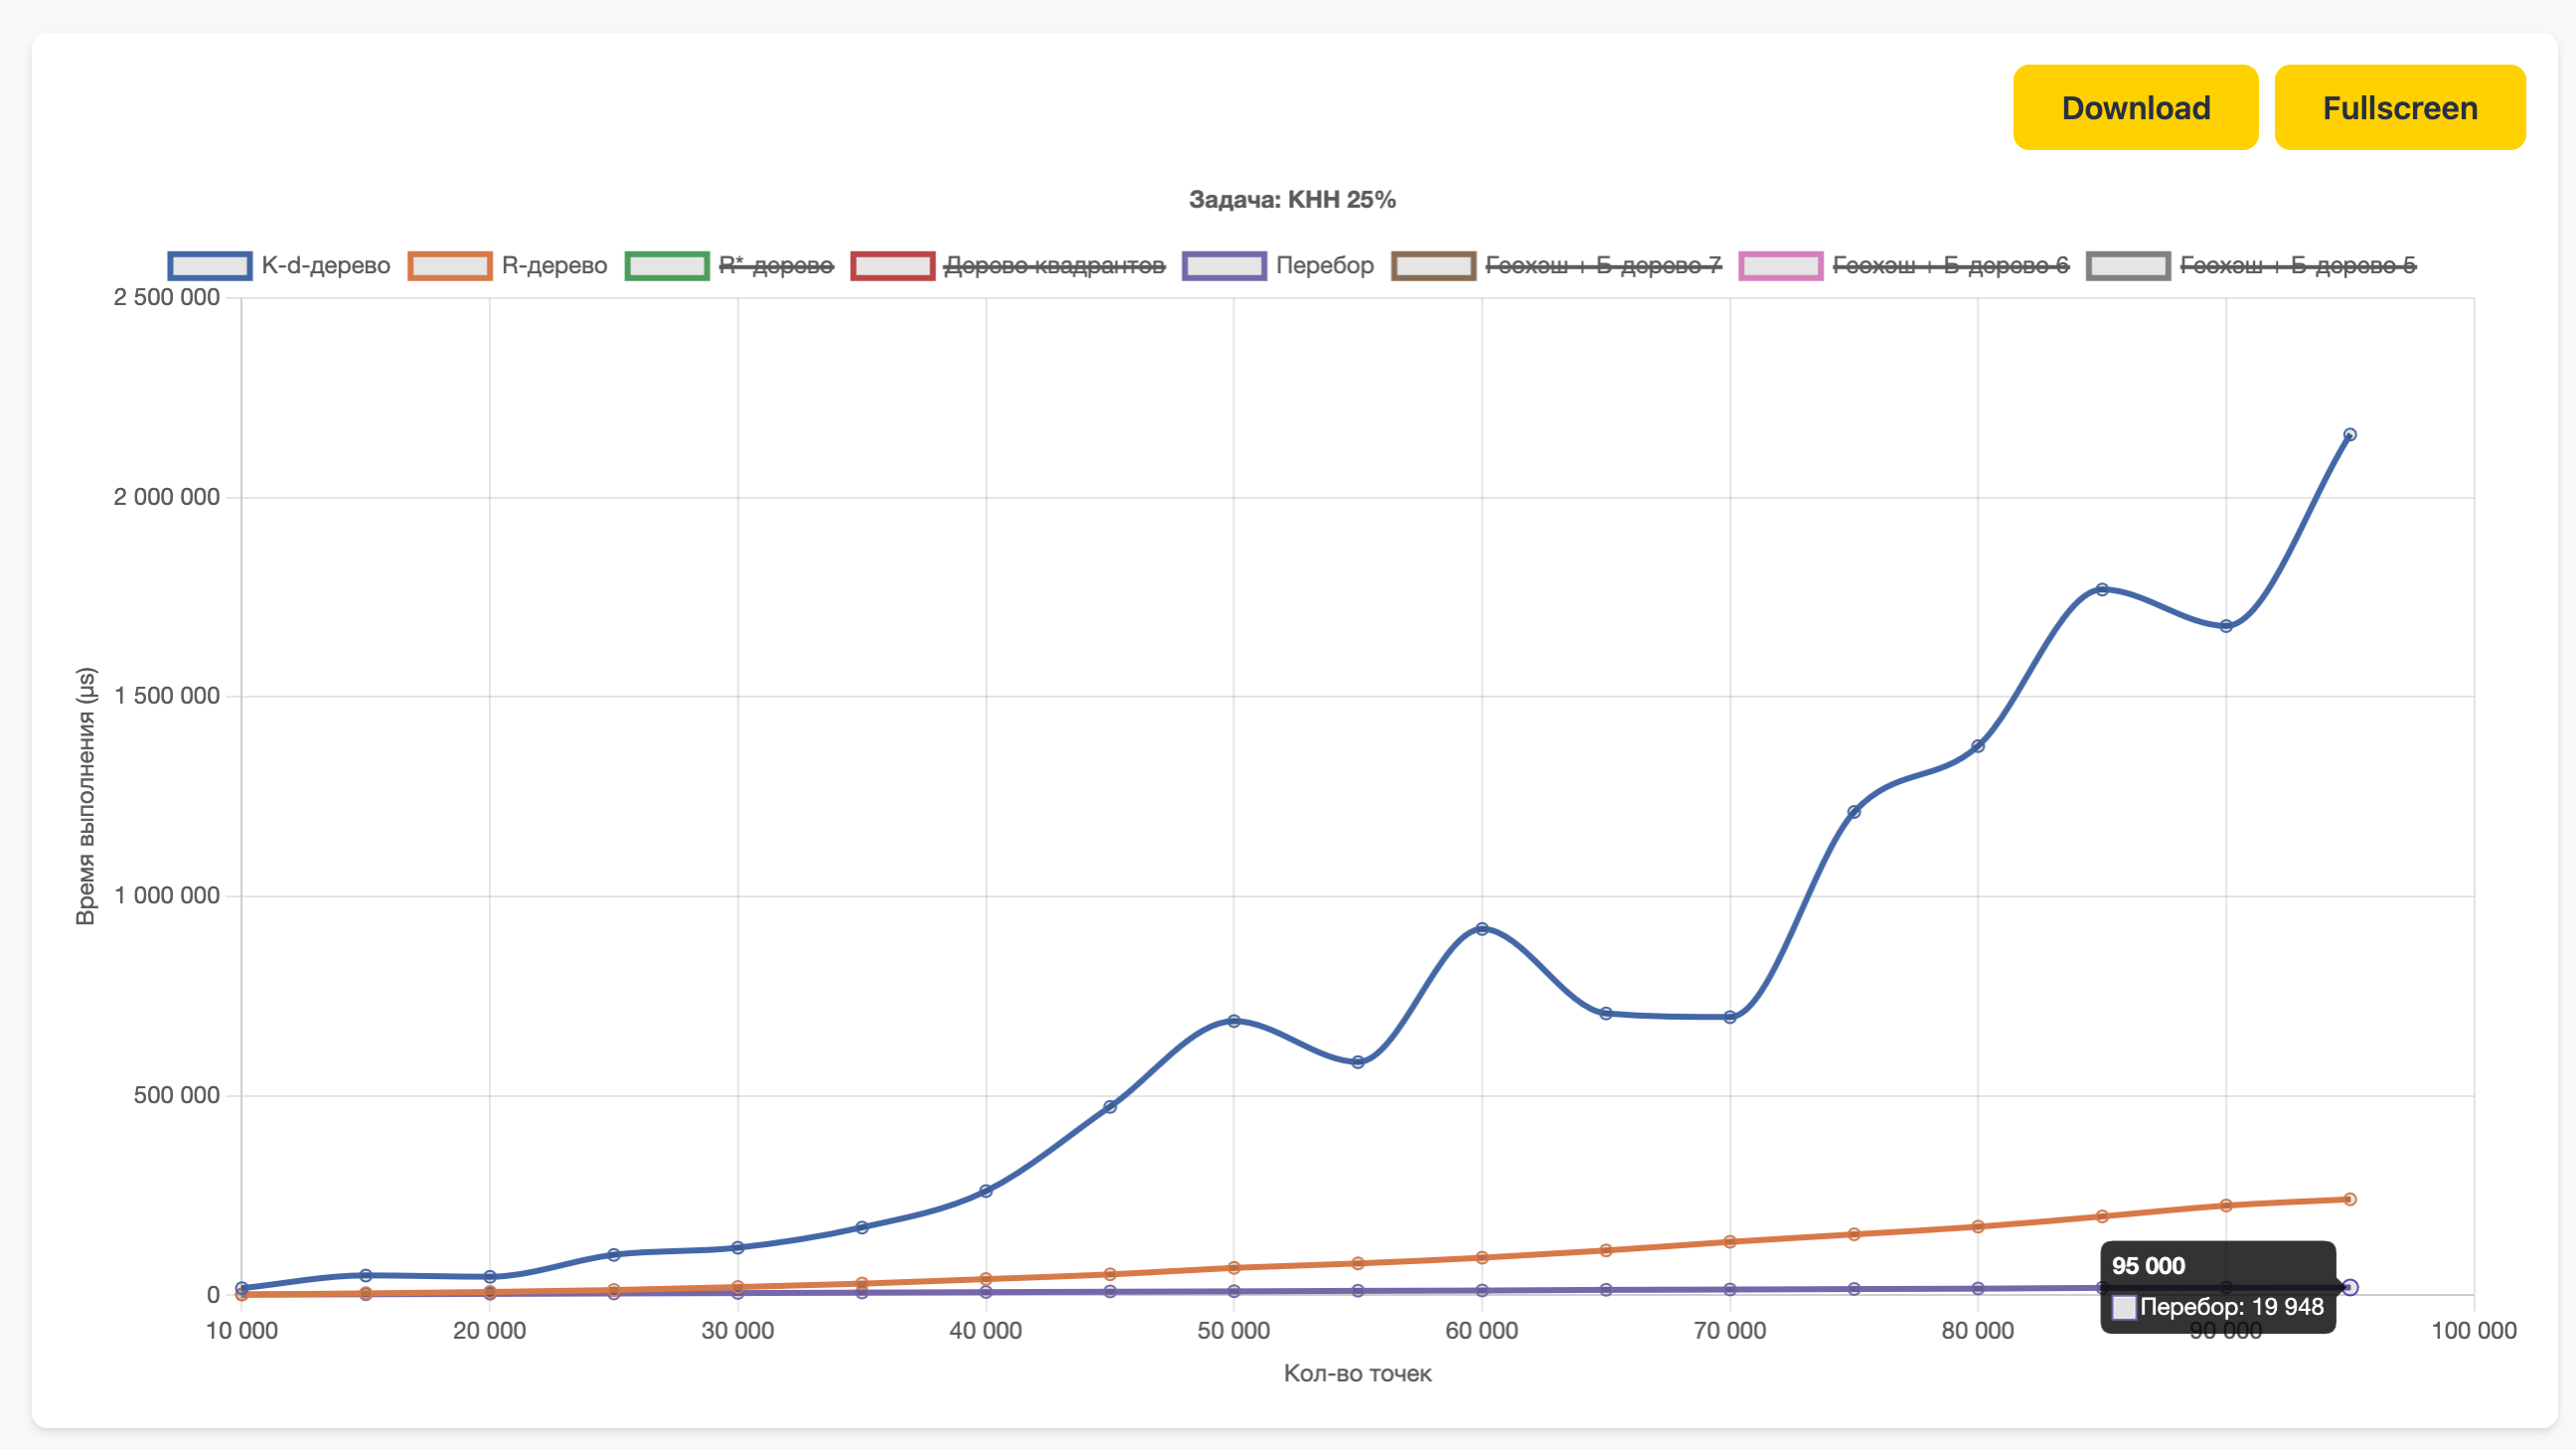
\includegraphics[scale=0.3]{result_knn_bruteforce.png}
    \caption{Результаты тестирования}
\end{figure}
\par\vspace{1em}
 
Иными словами, алгоритм простого перебора показывает хорошие результаты, когда K близко или сравнимо с N ($K \centernot \ll N$), что было взято за основу алгоритма «Geohash B-tree». 

Устройство разработанного «Geohash B-tree» тривиально, индекс представляет собой B-Tree\cite{comerBTree}, ключами которого являются геохеши в типе данных uint64, а значениями - массивы точек, которые находятся в указанном хеше. Размерность является параметром индекса и фиксируется. Для реализации алгоритмов поиска применяется возможность геохеша кластеризовать пространство земли и находить кластеры, в которых уже перебором производятся операции поиска по KNN или BBox\cite{gulakovStructured}.

Итерации поиска в прямоугольнике (рисунок 13):
\par а) получить геохеши углов, в примере на рисунке 13 --- \texttt{5} и \texttt{y} (если опускать общий префикс);
\par б) получить все точки, что находятся на гранях прямоугольника (\texttt{5}, \texttt{h}, \texttt{j}, \texttt{n} и тд.);
\par в) данные точки требуется также проверить на вхождение в прямоугольник через простой перебор;
\par г) все точки, что входят во внутрь (\texttt{k}, \texttt{s}, \texttt{m}, \texttt{t}), проверять не надо --- они гарантированно входят в прямоугольник.

\par\vspace{1em}
\begin{figure}[H]
    \centering
    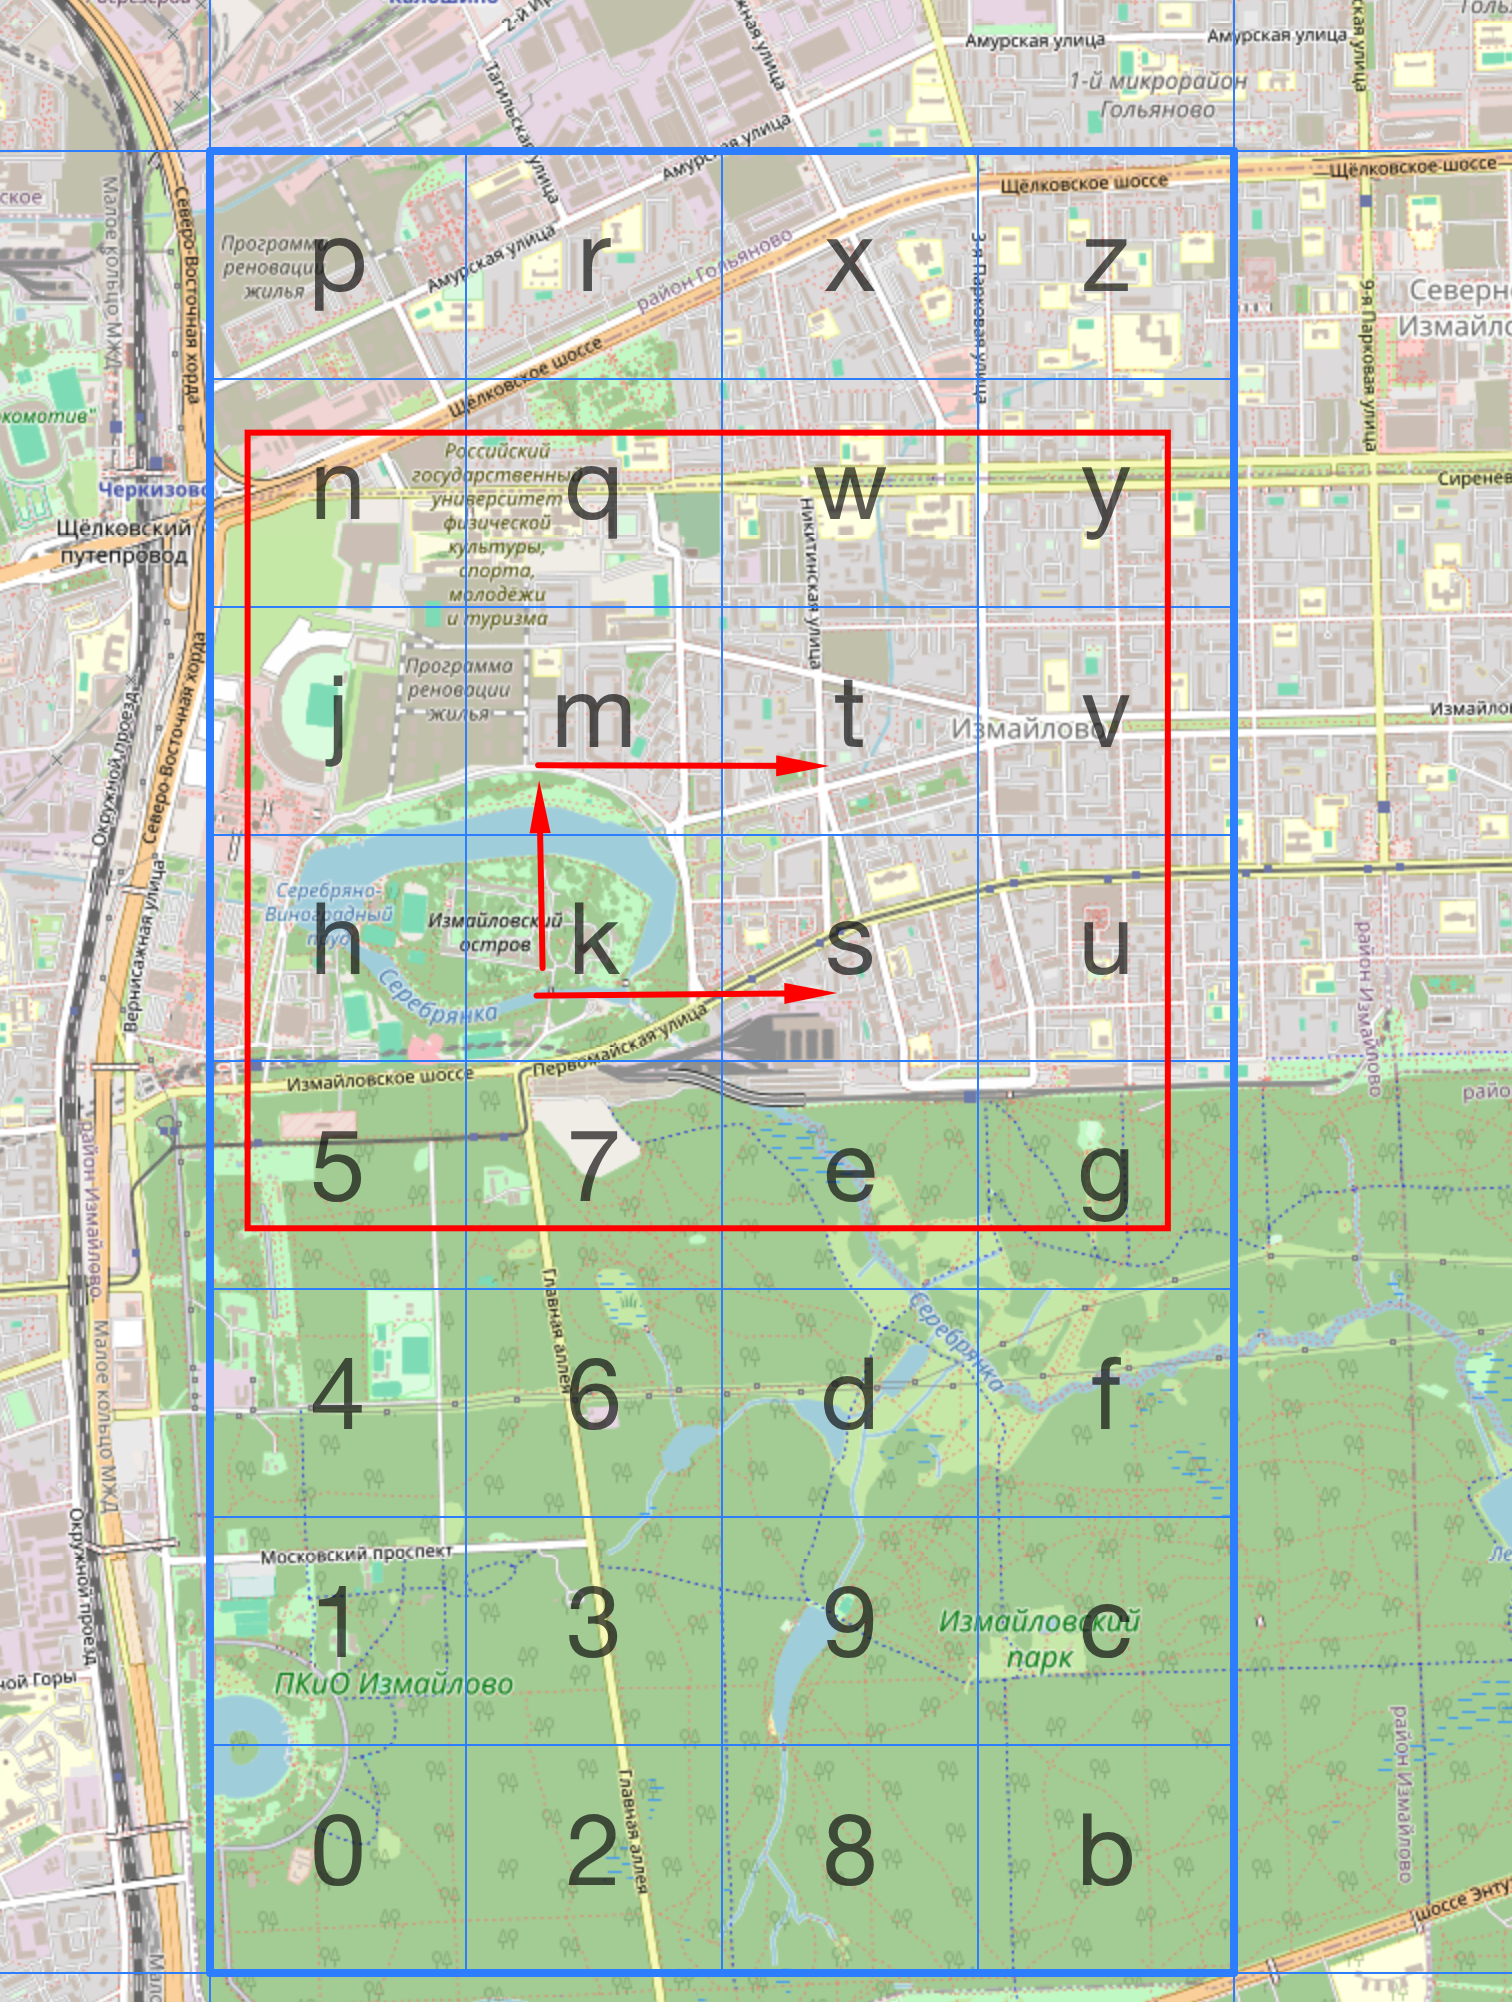
\includegraphics[scale=0.3]{geohash_btree_bbox.png}
    \caption{Алгоритм поиска в прямоугольнике}
\end{figure}
\par\vspace{1em}
  
Итерации поиска ближайшего соседа (рисунок 14):
\par а) найти геохеш точки P. В примере на рисунке 14 - \texttt{ucfv7m};
\par б) получить все точки, в указанном геохеше;
\par в) по часовой стрелке итерироваться по соседям оригинального геохеша и выгружать точки. (ucfv7m -> ucfv7q -> ucfv7w и тд);
\par г) завершить итерацию, когда кол-во найденных точек будет больше или равно K;
\par д) найти самую отдаленную точку из найденного массива относительно заданной точки P. Пусть расстояние между указанными точками будет R;
\par е) найти все точки в прямоугольнике, с центром в P и сторонами 2R;
\par ж) точки в полученном массиве отсортировать по расстоянию и выдать первые K точек.
  
\par\vspace{1em}
\begin{figure}[H]
    \centering
    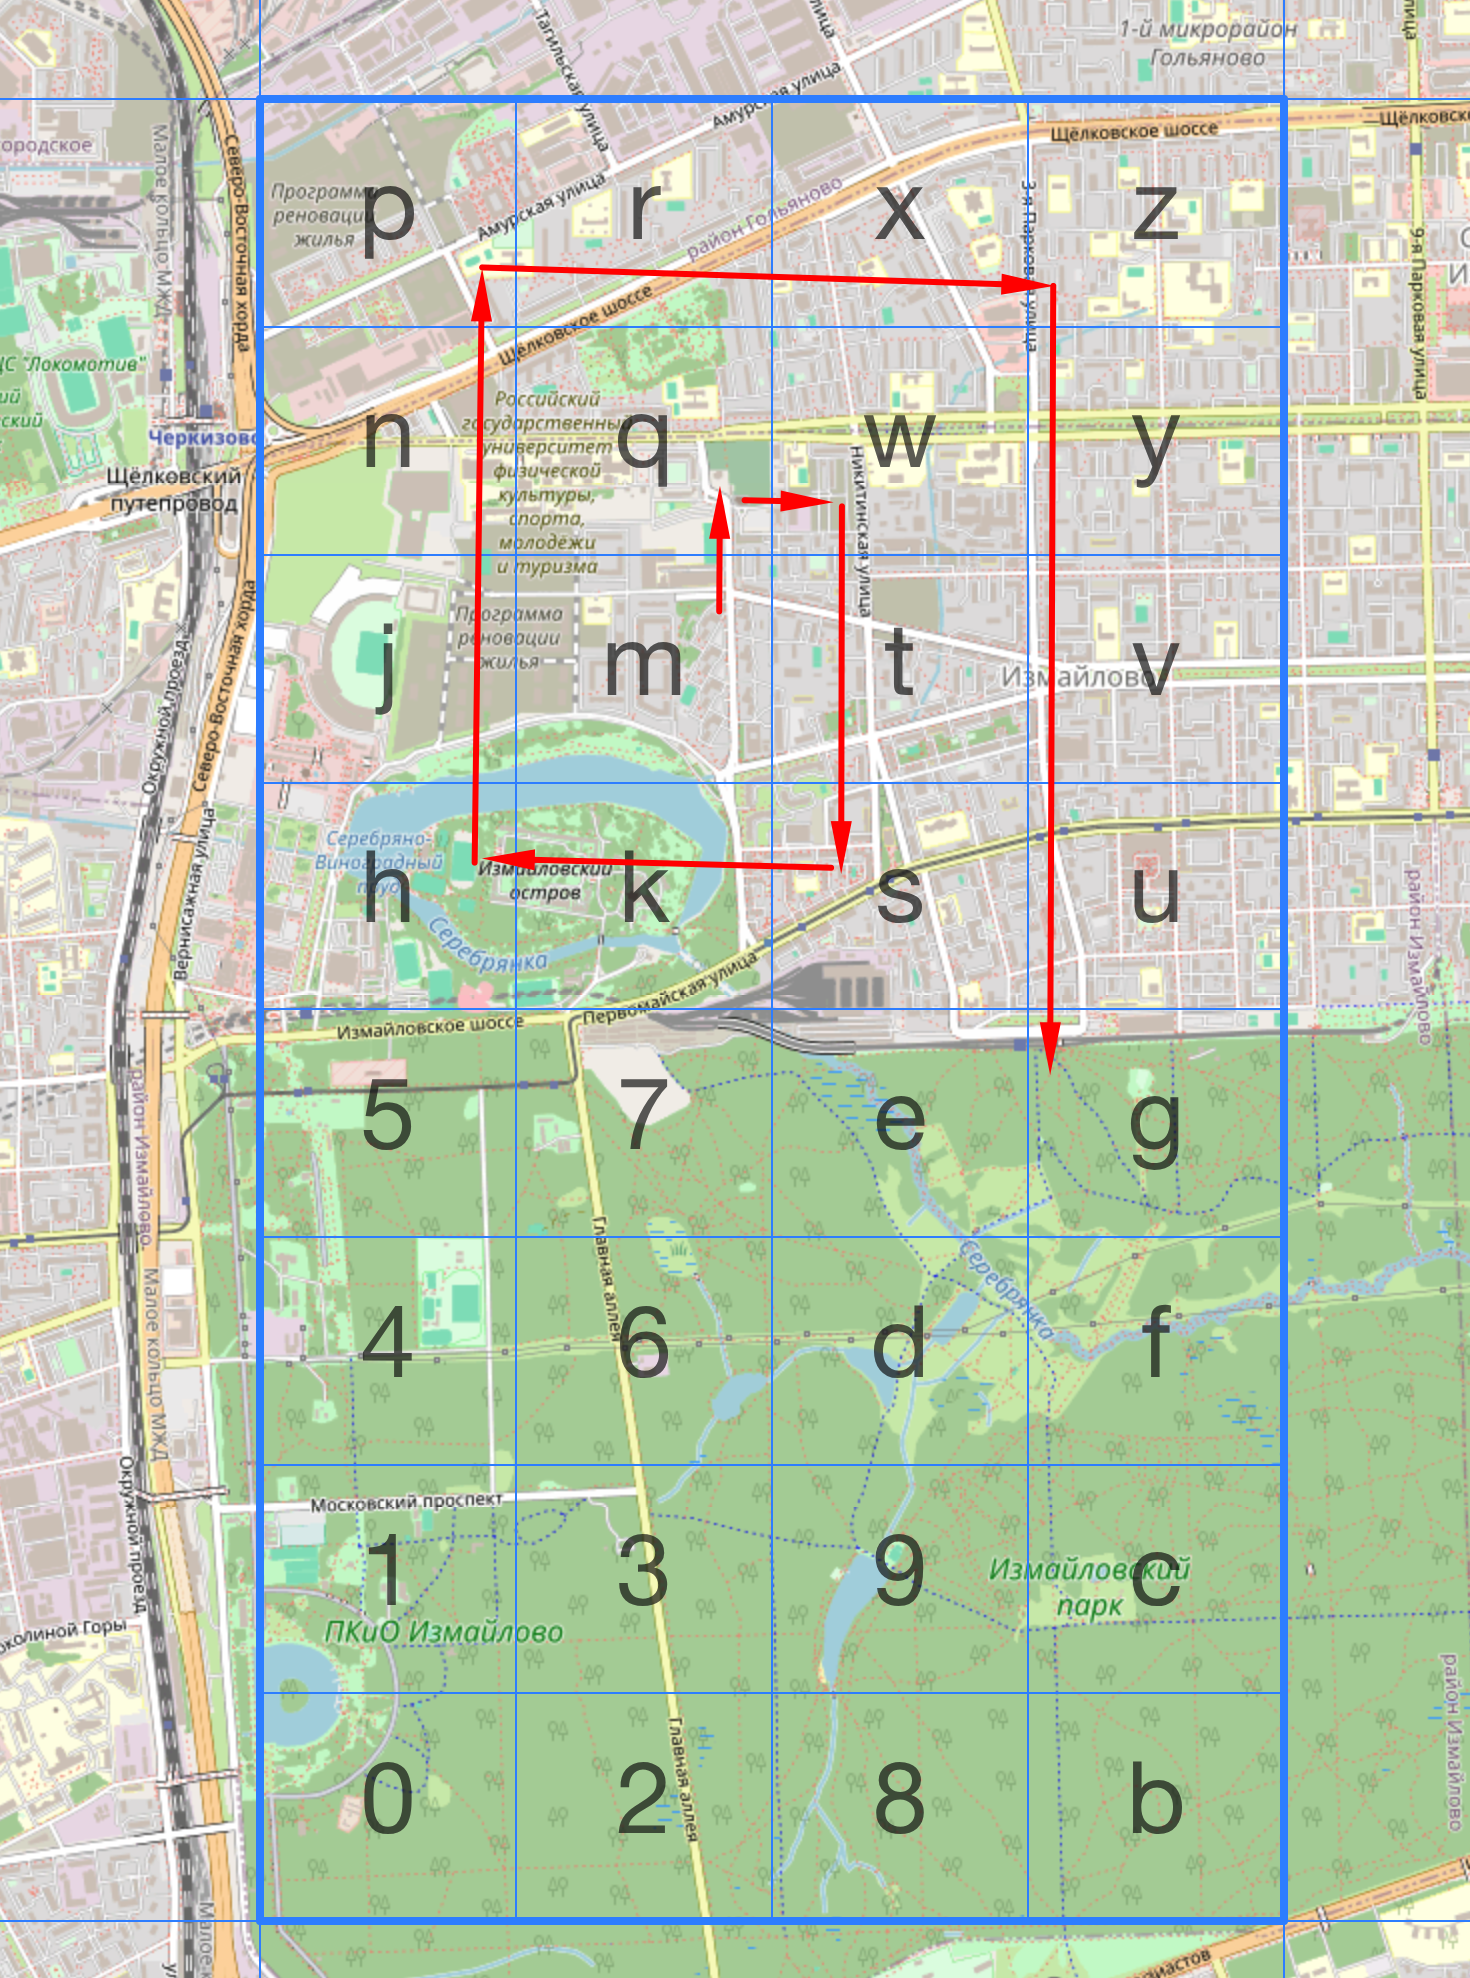
\includegraphics[scale=0.3]{geohash_btree_knn.png}
    \caption{Итеративный проход по соседям}
\end{figure}
\par\vspace{1em}
  
У разработанного алгоритма крайне много преимуществ:
\par а) клиентский. Может быть полностью реализован на стороне клиента, а не СУБД. Если СУБД не поддерживает какие-либо пространственные индексы, как например AWS DynamoDB, данный индекс можно использовать для закрытия потребности в пространственных индексах;
\par б) кластеризуемый. В отличие от R-Tree, данный индекс без проблем реализует кластеризацию. Также важно отметить, что B-Tree в данном индексе использует только операции Get и Set, без сравнения и итераций, за счет чего данный индекс можно применять, например, в СУБД Redis, которая нативно поддерживает кластеризацию ключей;
\par в) комбинируемый. В случае необходимости, его можно комбинировать с R-Tree, например, для СУБД Redis можно хранить в ключах хеши, а в значениях --- R-tree через операцию GEOADD\cite{redisGeo}. Тогда кластеризация останется доступной, при этом все методы R-Tree также сохранятся. 
    
Но также имеются минусы:
\par а) параметризируемость. На создании индекса требуется выбрать размерность Geohash, она не может быть изменена. Если выбранная размерность будет слишком большой или слишком малой, производительность индекса будет низкой;
\par б) крайние случаи. Если клиент отправит запрос на задачу KNN, при этом в указанной точке и рядом не будет точек, индекс будет медленно итерироваться по всем ближайшим геохешам.